98. \begin{figure}[ht!]
\center{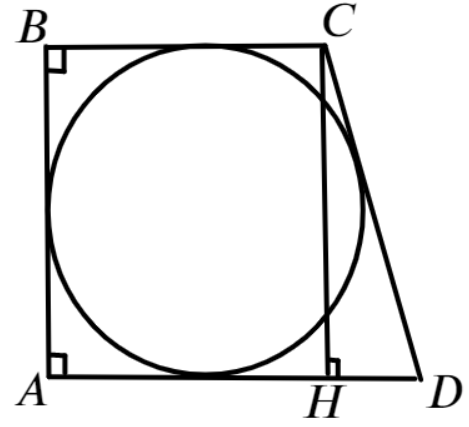
\includegraphics[scale=0.35]{g9-98.png}}
\end{figure}\\
Сторона $AB$ равна высоте трапеции и диаметру вписанной окружности, то есть $2R.$ Пусть $HD=x,$ тогда так как трапеция является описанной (суммы противоположных сторон равны), имеем $CD=\cfrac{4}{3}R+\cfrac{4}{3}R+x-2R=\cfrac{2}{3}R+x.$ По теореме Пифагора для треугольника $CHD$ получаем $x^2+4R^2=(x+\cfrac{2}{3}R)^2,\
x^2+4R^2=x^2+\cfrac{4}{3}xR+\cfrac{4}{9}R^2,\ x=\cfrac{8}{3}R,\ AD=\cfrac{4}{3}R+\cfrac{8}{3}R=4R, CD=\cfrac{2}{3}R+\cfrac{8}{3}R=\cfrac{10}{3}R.$ Таким образом,
стороны трапеции равны $2R,\ \cfrac{4}{3}R,\ \cfrac{10}{3}R,\ 4R.$\\
